\documentclass[10pt,a4paper,leqno]{article}         
\usepackage{CJKutf8}                          
\usepackage{inputenc}                         
\usepackage[T1]{fontenc}                      
\usepackage{amsmath,esint}                    
\usepackage{amsfonts}                         
\usepackage{amssymb}                          
\usepackage{xcolor}                           
\usepackage{mathrsfs}                         
\usepackage{makeidx}                          
\usepackage{graphicx}                         
\usepackage{float}                            
\usepackage{textcomp}                         
\usepackage{gensymb}                          
\usepackage{ifpdf}                            
\usepackage{tikz}                             
\usepackage[siunitx]{circuitikz}              
\usetikzlibrary{shapes,arrows,positioning,    
calc,patterns,decorations.pathmorphing,        
decorations.markings}                          
%\usepackage{tgothic}                         
\ifpdf                                        
\usepackage[breaklinks,hidelinks]{hyperref}   
\else                                         
\usepackage{url}                              
\fi                                           
%\newcommand*\VF[1]{\mathbf{#1}}              
%\newcommand*\dif{\mathop{}\!\mathrm{d}}      
\author{CBCO}                           
\title{Mechanical System Diagram in LaTeX Tikz}                             
\begin{document}                              
\maketitle

\noindent \newcommand\CWht[1][2.5]{\tikz[baseline=-#1]{\draw[thick](0,0)     circle[radius=1.5mm];}}
 \par \ \par\noindent \newcommand\CBlk[1][2.5]{\tikz[baseline=-#1]{\draw[thick,    fill=black!](0,0) circle[radius=1.5mm];}}
 \par \ \par\noindent \begin{CJK*}{UTF8}{gbsn}
 \par \ \par\noindent Exercise
 \par \ \par\noindent Use latex for all your drawing. See latex codes above for your referenc.
 \par \ \par\noindent 1. Draw the free body diagram of mechanical system shown in Figure 1 (b).
 \par \ \par\noindent 2. From your free body diagram, derive the equation of the mechanical system.
 \par \ \par\noindent 3. Rearrange your equation for control system block diagram. Generate the control system block diagram.
 \par \ \par\noindent \begin{figure}[H]\centering 

 \par \ \par\noindent 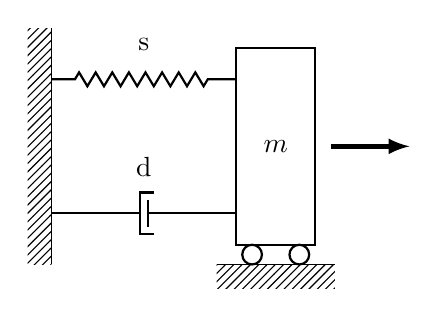
\begin{tikzpicture}[every node/.style={outer sep=0pt,thick}]              
\tikzstyle{spring}=[thick,decorate,decoration={zigzag,pre length=0.3cm,post   
length=0.3cm,segment length=6}]                                                
\tikzstyle{damper}=[thick,decoration={markings,mark connection node=dmp,      
mark=at position 0.5 with                                                      
{                                                                              
\node (dmp) [thick,inner sep=0pt,transform shape,rotate=-90,minimum           
width=15pt,minimum height=3pt,draw=none] {};                                   
\draw [thick] ($(dmp.north east)+(2pt,0)$) -- (dmp.south east) --             
(dmp.south west) -- ($(dmp.north west)+(2pt,0)$);                              
\draw [thick] ($(dmp.north)+(0,-5pt)$) -- ($(dmp.north)+(0,5pt)$);            
}                                                                              
}, decorate]                                                                   
\tikzstyle{ground}=[fill,pattern=north east lines,draw=none,minimum           
width=0.75cm,minimum height=0.3cm]                                             
            
%                                                                              
\begin{scope}[xshift=7cm]                                                     
\node (M) [draw,minimum width=1cm, minimum height=2.5cm] {$m$};               
\node (ground) [ground,anchor=north,yshift=-0.25cm,minimum width=1.5cm] at    
(M.south) {};                                                                  
\draw (ground.north east) -- (ground.north west);                             
\draw [thick] (M.south west) ++ (0.2cm,-0.125cm) circle (0.125cm)             
(M.south east) ++ (-0.2cm,-0.125cm) circle (0.125cm);                          
\node (wall) [ground, rotate=-90, minimum width=3cm,yshift=-3cm] {};          
\draw (wall.north east) -- (wall.north west);                                 
\draw [spring] (wall.170) -- node[above=.25]{s}($(M.north west)!(wall.170)!   
(M.south west)$);                                                              
\draw [damper] (wall.10) -- node[above=.35]{d}($(M.north west)!(wall.10)!     
(M.south west)$);                                                              
\draw [-latex,ultra thick] (M.east) ++ (0.2cm,0) -- +(1cm,0);                 
\end{scope}                                                                   
%                                                                              
                  
\end{tikzpicture}
 \par \ \par\noindent \caption{(b) Mechanical System Diagram} \end{figure}
 \par \ \par\noindent \begin{figure}[H]\centering 

 \par \ \par\noindent 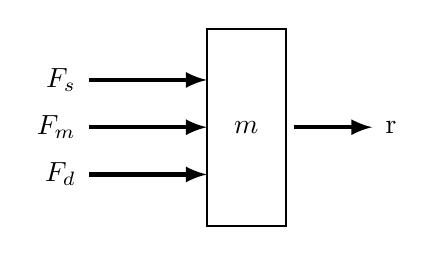
\begin{tikzpicture}[every node/.style={outer sep=0pt,thick}]              
\tikzstyle{spring}=[thick,decorate,decoration={zigzag,pre length=0.3cm,post   
length=0.3cm,segment length=6}]                                                
\tikzstyle{damper}=[thick,decoration={markings,mark connection node=dmp,      
mark=at position 0.5 with                                                      
{                                                                              
\node (dmp) [thick,inner sep=0pt,transform shape,rotate=-90,minimum           
width=15pt,minimum height=3pt,draw=none] {};                                   
\draw [thick] ($(dmp.north east)+(2pt,0)$) -- (dmp.south east) --             
(dmp.south west) -- ($(dmp.north west)+(2pt,0)$);                              
\draw [thick] ($(dmp.north)+(0,-5pt)$) -- ($(dmp.north)+(0,5pt)$);            
}                                                                              
}, decorate]                                                                   
\tikzstyle{ground}=[fill,pattern=north east lines,draw=none,minimum           
width=0.75cm,minimum height=0.3cm]                                             
\begin{scope}[xshift=7cm]                                                     
\node (M) [draw,minimum width=1cm, minimum height=2.5cm] {$m$};               
\draw [-latex,ultra thick] (M.east) ++ (0.1cm,0) -- +(1cm,0)node[right=.05cm]{r};                 
\draw [-latex,ultra thick] (-2cm,.6cm) node[left=.05cm]{$F_s$} -- (-.5cm,.6cm); 
\draw [-latex,ultra thick] (-2cm,0cm) node[left=.05cm]{$F_m$}-- (-.5cm,0cm); 
\draw [-latex,ultra thick] (-2cm,-.6cm)node[left=.05cm]{$F_d$} -- (-.5cm,-.6cm); 
\end{scope}                                                                   
\end{tikzpicture}
 \par \ \par\noindent \caption{(b) Free Body Diagram} \end{figure}
 \par \ \par\noindent Alternative Drawing.
 \par \ \par\begin{figure}[H]
\centering\includegraphics[width=1\linewidth,height=0.25\textheight]{Data/ExerciseFig.png}
\caption{Drawn using Paint Brush}
\label{fig:Data/ExerciseFig.png}
\end{figure}

\noindent \nocite{2}
 \par \ \par\noindent \nocite{201}
 \par \ \par\noindent \nocite{202}
 \par \ \par\noindent \nocite{301}
 \par \ \par\noindent \nocite{310}
 \par \ \par\noindent \bibliographystyle{plain} 
 \bibliography{ccoLib/ccobib}
 \par \ \par\noindent \end{CJK*}
 \par \ \par\end{document}